\newif\ifprint
%\printtrue % comment out to hide answers

\ifprint % print version
\documentclass[12pt,twoside]{fithesis2}
\else % pc version
\documentclass[12pt,oneside]{fithesis2}
\fi

% ===== LOADING PACKAGES =====
\usepackage[english, slovak ,czech]{babel}
% enabling new fonts support (nicer)
\usepackage{lmodern}
% setting input encoding
\usepackage[utf8]{inputenc}
% setting output encoding
\usepackage[T1]{fontenc}
% fithesis2 requires csquotes
\usepackage{cslatexquotes}
% set page margins
\ifprint % print version
\usepackage[top=3.0cm, bottom=3.5cm, left=2.9cm, right=1.9cm]{geometry}
\else % pc version
\usepackage[top=3.0cm, bottom=3.5cm, left=2.4cm, right=2.4cm]{geometry}
\fi
% package to make bullet list nicer
\usepackage{enumitem}
% math symbols and environments
\usepackage{mathtools}
% packages for complex tables
\usepackage{tabularx}
\usepackage{multirow}
\usepackage{siunitx}
\usepackage{dcolumn}
\usepackage{array}
% set italics style in floats captions to visually separate them from text
\usepackage[font=it]{caption}
% enable page rotation and floats rotation
\ifprint % print version
\usepackage[figuresright]{rotating}
\else % pc version
\usepackage{pdflscape}
\fi

%figures
\usepackage{float}
\restylefloat{figure}

\addto\captionsczech{
	\renewcommand{\figurename}{Obrázok.}
	\renewcommand{\listfigurename}{Zoznam obrázkov}
	\renewcommand{\listtablename}{Zoznam tabuliek}
	\renewcommand{\tablename}{Tabuľka}
}

% bibliography management
\usepackage[
    backend=biber,      % use biber as backend instead of BiBTeX
    style=alphabetic,   % citation style
	url=true,           % display urls in bibliography
	hyperref=auto,      % detect hyperref and create links
	sortlocale=cs_CZ,
	bibencoding=UTF8,
    firstinits=true,    % abbreviate first names to initials
    maxbibnames=5,      % maxiumim number of authors before making 'et al.'
    alldates=iso8601,   % set date format to ISO 8601
]{biblatex}

\bibliography{thesis}



% setting custom colors for links and table cells
\usepackage[table]{xcolor}
\definecolor{dark-red}{rgb}{0.6,0.15,0.15}
\definecolor{dark-green}{rgb}{0.15,0.4,0.15}
\definecolor{medium-blue}{rgb}{0,0,0.5}
% generating hyperlinks in document
\usepackage{url}
\usepackage[plainpages=false,   % get the page numbering correctly
            pdfpagelabels,      % write arabic labels to all pages
            unicode,           	% allow unicode characters in links
\ifprint % print version
            hidelinks,          % hide links
\else % pc version
            colorlinks=true,    % use colored links instead of boxed
\fi
            linkcolor={dark-red},
            citecolor={dark-green},
            urlcolor={medium-blue}
			]{hyperref}
% intelligent object references
\usepackage[nameinlink,noabbrev]{cleveref}

%titles
\usepackage{titlesec}

\titleformat{\chapter}[display]
{\bfseries\Large}
{\filright\MakeUppercase{\chaptertitlename} \Huge\thechapter}
{1ex}
{\titlerule\vspace{1ex}\filleft}
[\vspace{1ex}\titlerule]
\titleformat{\section}[hang]{
	\bfseries\Large}
{} 
{0em}
{\hspace{-0.4pt}\LARGE \thesection\hspace{0.6em}}

\titleformat{\subsection}[hang]{
	\bfseries\Large}
{} 
{0em}
{\Large \thesubsection\hspace{0.6em}}

\makeatletter
\def\ttl@mkchap@i#1#2#3#4#5#6#7{
	\ttl@assign\@tempskipa#3\relax\beforetitleunit
	\vspace{\@tempskipa}
	\global\@afterindenttrue
	\ifcase#5 \global\@afterindentfalse\fi
	\ttl@assign\@tempskipb#4\relax\aftertitleunit
	\ttl@topmode{\@tempskipb}{
		\ttl@select{#6}{#1}{#2}{#7}}
	\ttl@finmarks
	\@ifundefined{ttlp@#6}{}{\ttlp@write{#6}}}
\makeatother

% ===== MAIN DOCUMENT SETTINGS =====
% adjusting hyphenation penalties
\tolerance=10000
\hyphenpenalty=500
% renew command for shorter and nicer underscore
\renewcommand{\_}{\leavevmode \kern0.0em\vbox{\hrule width0.4em}}
% space between paragraphs
\setlength{\parskip}{0.6em plus0.2em minus0.2em}
% define square symbol
\newcommand{\squarebullet}{\textcolor{black}{\raisebox{0.15em}{\rule{4pt}{4pt}}}}
% define new itemize environment with squares and smaller spaces
\newenvironment{myItemize}{
  \begin{itemize}[leftmargin=2em,rightmargin=1em,itemsep=0.75\parskip,parsep=0em,topsep=0em,partopsep=0em]
  \renewcommand{\labelitemi}{\squarebullet}
  \renewcommand{\labelitemii}{$\diamond$}
}{
  \end{itemize}
}
% define new enumerate environment with smaller spaces
\newenvironment{myEnumerate}{
  \begin{enumerate}[leftmargin=2em,rightmargin=1em,itemsep=0.75\parskip,parsep=0em,topsep=0em,partopsep=0em]
}{
  \end{enumerate}
}
% FI THESIS settings
\thesistitle{Rozšírenie frameworku EACirc o simulátor Java bytecodu}
\thesissubtitle{Bakalárska práca}
\thesisstudent{Michal Hajas}
\thesiswoman{false}
\thesisfaculty{fi}
\thesisyear{jar 2016}
\thesisadvisor{Ing. Mgr. et Mgr. Zdeněk Říha, Ph.D}
\thesislang{sk}

% ===== NEW COMMANDS =====
% macro for quotes mimicking czech/slovak babel
% \newcommand\uv[1]{\quotedblbase #1\textquotedblleft}
% full-page landscape table (print conditioned compilation)
\newcommand{\fullPageLandscapeTable}[1]{
\ifprint % print version
\begin{sidewaystable}
\else % pc version
\begin{landscape}
\begin{table}[p]
\fi
\centering
#1
\ifprint % print version
\end{sidewaystable}
\else % pc version
\end{table}
\end{landscape}
\fi
}
% new table column types with flexible width
\newcolumntype{C}{>{\centering\arraybackslash}X}
\newcolumntype{R}{>{\raggedleft\arraybackslash}X}
% rotated (one or multi line) table cell
\newcommand{\rotatedHeader}[2][l]{\rotatebox{90}{\renewcommand{\arraystretch}{0.75}\begin{tabular}[#1]{@{}l}#2\end{tabular}}}
% shorthands for coloured cells
\newcommand{\cc}{\cellcolor{black!10}}  % light gray background
% shorthand for star symbol in tables
\newcommand{\st}{$^{\star}$}
% header for results tables
\newcommand{\resultsTable}[4]{%
\small
 \begin{table}[h]
 	
 	\renewcommand{\arraystretch}{1.2}
 	\small
 	\begin{tabularx}{\textwidth}{|C||C|C|C|C|C|}
 		\hline
 		\multicolumn{6}{|c|}{\textbf{#1}} \\
 		\hline \hline
 		\vspace{5pt}
		\textbf{Runda} &
 		\vspace{0pt}
 		\begin{tabular}[b]{@{}c}\small\textbf{Bežné uzly} \\ \scriptsize(proportion) \end{tabular} &
		\vspace{0pt}
 		\begin{tabular}[b]{@{}c}\small\textbf{Tangle} \\ \scriptsize(proportion) \end{tabular} &
		\vspace{-10pt}
 		\begin{tabular}[b]{@{}c}\small\textbf{Dynamic} \\ \small\textbf{SHA} \\ \scriptsize(proportion) \end{tabular} &
		\vspace{-10pt}
 		\begin{tabular}[b]{@{}c}\small\textbf{Dynamic} \\ \small\textbf{SHA-2} \\ \scriptsize(proportion) \end{tabular} &
 		\vspace{0pt}
 		\begin{tabular}[b]{@{}c}\small\textbf{Decim} \\ \scriptsize(proportion) \end{tabular} \\
 		\hline\hline
 		#2
 		\hline
 		
 	\end{tabularx}
 	\caption{#3}
 	\label{#4}
 \end{table}
}

% two column part
\newcommand{\twoColumns}[2]{%
	\begin{minipage}{0.47\textwidth}
		\centering
		#1
	\end{minipage}
	\hfill
	\begin{minipage}{0.47\textwidth}
		\centering
		#2
	\end{minipage}
}





% ===== NAME MACROS =====
\newcommand{\eacirc}{EACirc}
\newcommand{\niststs}{NIST STS}
\newcommand{\dieharder}{Dieharder}
\newcommand{\testu}{TestU01}
\newcommand{\caesar}{CAESAR}

% ===== BEGIN DOCUMENT =====
\begin{document}

\FrontMatter
%\ThesisTitlePage

%\begin{ThesisDeclaration}
%\DeclarationText
%\AdvisorName
%\end{ThesisDeclaration}

%\begin{ThesisThanks}
%Many thanks to you all.

%\end{ThesisThanks}

%\begin{ThesisAbstract}
%Abstrakt
%\end{ThesisAbstract}

%\begin{ThesisKeyWords}
%Klucove slova
%\end{ThesisKeyWords}

\MainMatter
%\tableofcontents

%\chapter*{Úvod}
\label{chap:introduction}
\addcontentsline{toc}{chapter}{\textbf{Úvod}}
Uvod

\chapter{Štatistické testovanie náhodnosti}
\label{chap:statistic-tests}

Náhodné dáta zohrávajú dôležitú úlohu v rôznych odvetviach informatiky. Veľkú rolu majú napríklad v kryptografii, pretože jedným z požiadavkov na zašifrované dáta je aj nemožnosť zistiť, či sú výstupom zo šifrovacej funkcie, alebo len náhodná sekvencia. Aby sme vedeli rozoznať, či šifrovacia funkcia spĺňa toto kritérium, potrebujeme nástroj, ktorým keď preskúmame dáta zistíme, či sú náhodné alebo nie. Avšak zistiť, či sú dáta náhodné nie je vôbec jednoduché, pretože vlastnosť naozaj náhodného generátora je, že vygeneruje každú sekvenciu s rovnakou pravdepodobnosťou. To znamená, že každá sekvencia môže byť výstupom z náhodného generátora.

Najrozšírenejším nástrojom na testovanie náhodnosti sú tzv. štatistické sady často nazývané aj štatistické batérie. Každá sada pozostáva z viacerých testov, kde každý test skúma požadovanú vlastnosť na vstupných dátach. Z každého spusteného testu je výstupom výsledok, ktorý je následne spolu s výsledkami ostatných testov skombinovaný. Keďže sa nikdy nedá určiť, či sú dáta náhodné alebo nie na 100 percent, tak výsledok nemôže byť formou áno respektíve nie. Preto sa výsledok vyjadruje iba ako pravdepodobnosť s akou by naozaj náhodný generátor vygeneroval menej náhodné dáta ako testované dáta \cite{nist-sts-interpretation-syso}. 

\section{NIST STS}
\label{sec:sts-nist}

Najznámejšia zo štatistických sád na štatistické testovanie náhodnosti \textit{Statistical Test Suite for Random and Pseudorandom Number Generators for Cryptographic Applications}~\parencite{nist-sts-documentation}, ktorá vznikla v Národnom inštitúte štandardov a technológií (NIST), používa vo svojej testovacej sade množinu 15-tich testov, ktoré boli zostavené na základe predstavy o tom, ako by mala náhodná sekvencia vyzerať. Napríklad pre každú sekvenciu vygenerovanú náhodným generátorom platí, že pri zápise v binárnej sústave je na každej pozícií s rovnakou pravdepodobnosťou 1 alebo 0. Preto je napríklad malá pravdepodobnosť, že naozaj náhodná sekvencia bude obsahovať len samé jednotky, naopak s oveľa vyššou pravdepodobnosťou bude počet 1 a 0 približne rovnaký. Z tohto dôvodu je jedným z testov, ktorý obsahujú štatistické sady aj test, ktorý testuje či je táto vlastnosť splnená. Niektoré z testov majú dokonca možnosť nastaviť parametre, vďaka ktorým sa môže nad dátami spustiť tento test vo viacerých variantách. To znamená, že konečný počet spustených testov môže byť niekoľko násobne väčší ako počet testov, ktoré sada obsahuje. Cez rozhranie na príkazovom riadku sa dá pred spustením nastaviť kombinácia testov podľa toho, aké výsledky chceme získať. Avšak interpretácia výsledkov nie je triviálna. Každý test sa spustí nad viacerými sekvenciami. Ako výsledok testu, pre každú sekvenciu je p-hodnota z~intervalu $[0, 1]$, ktorá značí pravdepodobnosť, že by naozaj náhodný generátor vygeneroval menej náhodnú sekvenciu. Napríklad pre 1000 sekvencií dostaneme ku každému testu 1000 p-hodnôt. Na určenie výsledku sa používajú 2 metódy:
\begin{myItemize}
	\item \textbf{Uniformné rozloženie p-hodnôt po celom intervale $[0, 1]$}\\Na to aby sa dáta dali považovať za náhodné by mali byť všetky p-hodnoty rovnomerne rozdelené po celom intervale $[0, 1]$. To znamená, že keď bude interval rozdelený na 10 častí podľa hodnoty, teda prvá časť bude obsahovať p-hodnoty z~intervalu $[0, 0.1]$, druhá časť p-hodnoty z~intervalu $[0.1, 0.2]$ atď. malo by v každej časti skončiť rovnaké množstvo p-hodnôt, v našom prípade približne 100.
	\item \textbf{Pomer úspešných testov ku všetkým testom}\\Ďalší spôsob na určovanie výsledku je pomer úspešných testov. Na určenie výsledku potrebujeme hodnotu hladiny významnosti ($\alpha$) a interval do ktorého musí pomer spadnúť (interval je vypočítaný na základe hodnoty $\alpha$). Každá z 1000 p-hodnôt získaná z jedného testu je porovnaná s hodnotou $\alpha$. Ak je hodnota menšia, test pre jednu sekvenciu neprešiel. Ak je väčšia, test prešiel. Pomer počtu sekvencií, ktoré testami prešli, ku počtu všetkých testovaných sekvencií, by mal ležať vo vypočítanom intervale.
\end{myItemize}
Podľa článku \textit{On the Interpretation of Results from the NIST Statistical Test Suite}~\parencite{nist-sts-interpretation-syso} je vysoká pravdepodobnosť, až 80\%, že aj výstup z naozaj náhodného generátora neprejde niekoľkými testami. Autori spomenutého článku ukázali, že dáta sa dajú považovať za náhodné aj vtedy, ak neprejde (to znamená p-hodnota je menšia ako $\alpha$ = 1\%) 6 testov. Autori v článku si na testovanie zvolili množinu 188 testov.

\section{Dieharder}
\label{sec:dieharder}
Dieharder~\parencite{dieharder} je sada vytvorená Robertom G. Brownom na Duke univerzite za účelom zrýchliť a zjednodušiť spúšťanie testov tak, aby ich mohol rýchlo a jednoducho spustiť každý, kto potrebuje o svojich dátach zistiť, či sú náhodné. Testovacia sada je následníkom Diehard-u~\parencite{diehard}, avšak testy sú upravené a začlenené do rovnakej štruktúry. Taktiež sú do nej pridané testy z iných sád alebo od iných samostatných autorov. Vo verzii 3.31.1 z~roku 2003 sa nachádza 31 testov, z toho 17 pochádza z pôvodnej sady Diehard, 3 zo sady STS NIST (autori očakávajú, že raz bude obsahovať všetky testy) a zvyšných 11 z rôznych zdrojov, napríklad aj od samotného autora R. G. Browna.

\section{TestU01}
\label{sec:testu01}
Tvorcom Test-U01~\parencite{testu01} je  Pierre L’Ecuyer, ktorý pôsobí na univerzite v Montreale. Táto sada obsahuje množstvo testov, ktoré sa dajú spúšťať rôznymi spôsobmi, napríklad prostredníctvom batérií, čo sú v podstate skupiny testov, alebo samostatne. Testy sú implementované v jazyku ANSI C. Knižnica je rozdelená do viacerých modulov, ktorých popis je k dispozícii v dokumentácii~\parencite{testu01-documentation} a jedným z nich sú aj testovacie batérie. Sada obsahuje viac batérii testov, kde každá batéria má svoje určenie.
\begin{myItemize}
	\item \textbf{Small crush}\\Vytvorená tak, aby čo najrýchlejšie poskytla výsledok a preto neobsahuje veľa testov. Slúži na testovanie generátorov náhodných sekvencií.
	\item \textbf{Crush}\\Narozdiel od Small crush obsahuje viac testov. Zaberie teda viac času, avšak ak všetky testy prejdú, môžme si byť istejší pravdivosťou výsledku. Takisto ako small crush, aj crush slúži na testovanie generátorov.
	\item \textbf{Big crush}\\Ešte väčšia a pomalšia batéria ako crush a small crush. 
	\item \textbf{Alphabit}\\Primárne určená na hardware generátory, na vstupe môže brať aj jeden binárny súbor.
	\item \textbf{Rabbit}\\Takisto ako Alphabit môže mať ako vstup binárny súbor.
	\item \textbf{A ďalšie}\\Obsahuje batérie, ktoré simulujú batérie spomenuté vyššie, napríklad PseudoDIEHARD, ktorá simuluje batériu DIEHARD~\parencite{diehard} alebo batéria FIPS\_140\_2, ktorá napodobňuje STS od NIST.	 
\end{myItemize}

\chapter{Framework EACirc}
\label{chap:eacirc}

Testovanie náhodnosti štatistickými testami (\hyperref[chap:statistic-tests]{kapitola 1}) má však aj svoje nevýhody. Pre zjednodušenie si predstavme, že sa v batérii nachádza iba jeden test, ktorý testuje, či je počet núl a jednotiek približne rovnaký. Potom nie je zložité vytvoriť sekvenciu, ktorá testom prejde, napríklad postupnosť, v ktorej sa pravidelne striedajú nuly a jednotky, avšak je veľmi malá pravdepodobnosť, že by takáto sekvencia bola výstupom z naozaj náhodného generátora. Nevýhodou štatistických sád je, že testy, ktoré obsahujú, dokážu odhaliť iba nezrovnalosti, na ktoré boli naprogramované. Preto sa v štatistických sadách nachádza veľké množstvo testov, avšak každý test pridáva iba jednu vlastnosť, ktorú kontroluje. Avšak náhodnosť, neznamená spĺňať presne danú množinu vlastností. Z toho vyplýva, že výsledok zo štatistických testov nemusí vždy garantovať, že sú dáta naozaj náhodné respektíve nenáhodné. Tento nedostatok rieši alternatívny prístup, \textit{Framework EACirc}~\parencite{ukrop-bc}. 

Prístup EACircu je oproti štatistickým testom úplne odlišný. Nesnaží sa priamo určiť či sú skúmané dáta náhodné, namiesto toho hľadá funkciu, ktorá určí či na vstupe dostala naozaj náhodné dáta, alebo skúmané dáta. Na základe nájdenia respektíve nenájdenia takejto funkcie vyhlasuje, či sú skúmané dáta náhodné. Z toho vyplýva, že použitie kvalitných náhodných dát, je veľmi dôležitou súčasťou EACircu.

\section{Princíp fungovania}
\label{sec:principle}

Vytváranie hore zmienenej funkcie pripomína pomyselnú skladačku. Zatiaľ čo štatistické testy sa dajú prirovnať k hotovej skladačke, s ktorou sa nedá hýbať. EACirc obsahuje iba samotné komponenty, z ktorých sa dá výsledná skladačka poskladať akýmkoľvek spôsobom. Najdôležitejšou úlohou EACircu je zložiť tieto komponenty do jedného celku tak, aby výsledná skladačka splňovala požadované vlastnosti, teda aby funkcia opísaná touto skladačkou vedela rozlišovať medzi náhodnými dátami a skúmanými dátami. Na poskladanie používa samovzdelávací, genetický algoritmus (detailný pohľad v \hyperref[sec:genetics]{sekcii 2.2}), ktorý najprv náhodne poskladá ľubovoľné kocky na seba a potom sa skladačku snaží malými zmenami vylepšovať.

Cieľom EACircu je využiť tento prístup na to, aby ním z jednoduchých funkcií (vysvetlenie funkcií v \hyperref[sec:nodes]{sekcii 2.3}) vytvoril postupnosť, ktorá dokáže rozlíšiť či na vstupe dostala náhodné dáta. S týmto prístupom sa spája viac výhod, napríklad:
\begin{myItemize}
	\item \textbf{Na vytváranie testov nie je potrebná žiadna ľudská aktivita}\\Testy zo štatistických sád bývajú založené na matematických problémoch, nad ktorými museli ľudia stráviť množstvo času.
	\item \textbf{Testovanie aj zatiaľ nepoznaných problémov}\\Neexistujú testy na všetky vlastnosti nenáhodných dát, ale EACirc dokáže testovať teoreticky čokoľvek k čomu genetika dospeje.
\end{myItemize}

Takisto ako niektoré štatistické batérie (\hyperref[chap:statistic-tests]{kapitola 1.}), aj EACirc obsahuje integrované generátory prúdov dát, napríklad niekoľko hašovacích funkcií z rodiny SHA3~\parencite{thesis-dubovec}, alebo prúdové šifry eStream~\parencite{thesis-pristak}. Tiež obsahuje kandidátov zo súťaže CAESAR, ktorých pridal vo svojej {diplomovej práci}~\parencite{ukrop-master} Martin Ukrop. EACirc potrebuje na svoj beh XML súbor v ktorom sa nachádza konfigurácia, napríklad nastavenie prúdov, počet rúnd atď. Preto Ľubomír Obrátil vytvoril nástroj OneClick~\parencite{obratil-bc}. Ako už predznamenáva názov, jedná sa o nástroj, ktorý zjednodušuje prácu s EACircom, napríklad generuje konfiguračné súbory alebo vyhodnocuje výsledky. EACirc podporuje aj zrýchlenie výpočtu pomocou nVidia CUDA technológie, toto rozšírenie doplnil vo svojej {bakalárskej práci}~\parencite{novotny-bc} Jiří Novotný. 

\section{Genetika}
\label{sec:genetics}

Algoritmus použitý v EACircu je založený na biologicky inšpirovanom samovzdelávacom algoritme. V tejto kapitole si objasníme princíp načrtnutý v \hyperref[sec:nodes]{sekcii 2.1}. Kocky skladačky sú v skutočnosti uzly grafu, spojiť dve kocky znamená vytvoriť medzi nimi v grafe cestu. Graf je rozdelený do horizontálnych vrstiev, ktoré sú poskladané na seba, kde v každej z nich sa nachádza niekoľko uzlov. Cesty vedú len smerom zhora nadol, a to len medzi vrstvami idúcimi bezprostredne za sebou (\hyperref[obr:circuit-example]{obrázok 2.1}). Prvá vrstva je vstupná a posledná výstupná. Keďže sa jedná o biologický algoritmus tento graf sa tiež označuje pojmom jedinec alebo obvod.

\begin{figure}[h!]
	\centering
	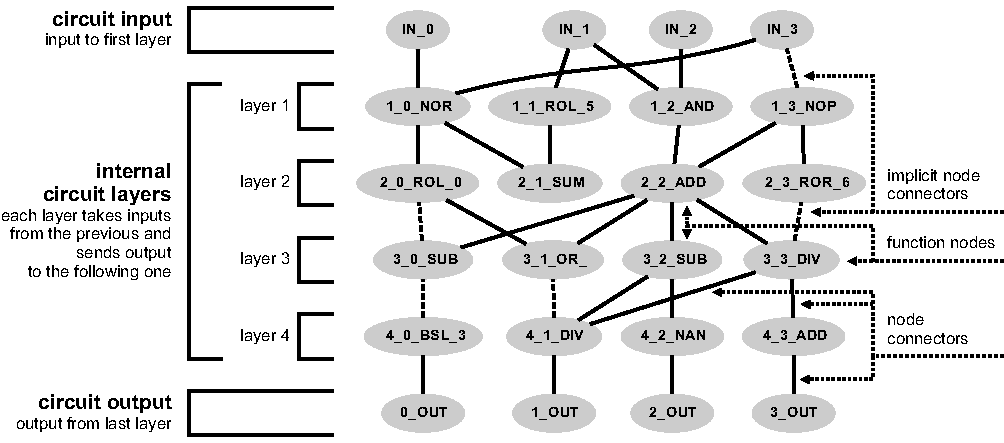
\includegraphics[scale=0.8]{./img/circuit-final.pdf}
	\caption{Vizualizáciu obvodu z {bakalárskej práce}~\parencite{ukrop-bc} Martina Ukropa.}
	\label{obr:circuit-example}
\end{figure}

Celý priebeh algoritmu spočíva v nasledujúcich krokoch:\vspace{-10pt}
\begin{enumerate}
	\item \textbf{Náhodné vygenerovanie obvodov}\\Vytvorí sa tzv. populácia náhodných jedincov. Veľa z nich bude neúspešných, avšak nájdu sa aj takí, ktorí budú od ostatných lepší. 
	\item \textbf{Určenie úspešnosti}\\Úspešnosť sa vypočíta pomocou tzv. funkcie vhodnosti, ktorá je pre správny priebeh veľmi dôležitá.
	\item \textbf{Vyradenie neúspešných obvodov}
	\item \textbf{Sexuálne skríženie najúspešnejších jedincov}\\Skrížením dostaneme novú populáciu jedincov. Cieľom kríženia je dosiahnuť novú silnejšiu generáciu, založenú len na tých najlepších jedincoch z predchádzajúcej populácie.
	\item \textbf{Náhodná mutácia niektorých jedincov}\\Aby sa zabránilo zaseknutiu sa v lokálnom maxime, je potrebné urobiť nejakú náhodnú mutáciu, napríklad odobrať cestu, alebo zmeniť niektorý z uzlov. Mutácia prebieha tak, že sa postupne prechádza obvodom a pri každom uzle respektíve hrane sa z nejakou pravdepodobnosťou vykoná mutácia.
	\item Kroky 2-5 su prevádzané v cykle až kým sa nedosiahne požadovaná úspešnosť alebo kým sa nevyčerpá určený počet generácií.
\end{enumerate}
Podstata genetiky je nájsť obvod, ktorý vie rozlišovať medzi naozaj náhodnými dátami a skúmanými dátami. Ak sa takýto obvod nájde, znamená to, že EACirc objavil v skúmaných dátach niečo, čo sa v naozaj náhodných dátach vyskytuje zriedkavo. To znamená, že dáta zrejme nebudú náhodné.

\section{Typy uzlov}
\label{sec:nodes}

V tejto sekcii si vysvetlíme aká je vlastne podstata samotného fungovania obvodov. Ako už bolo spomenuté v \hyperref[sec:genetics]{sekcii 2.2} každý jedinec sa skladá z horizontálnych vrstiev, kde v každej vrstve sa nachádzajú uzly. Každý uzol nesie v sebe informáciu, uloženú na 4 Bytoch, kde na prvom byte je uložené číslo funkcie ktorá sa má vykonať. Na ostatných miestach sú potom uložené voliteľné parametre. Avšak nie všetky funkcie tieto parametre využívajú. Jedná sa o nasledujúce funkcie:

\begin{myItemize}
	\item \textbf{Bitové operátory}\\AND, OR, XOR, NOR, NAND, ROTL, ROTR, BITSELECTOR
	\item \textbf{Aritmetické funkcie}\\SUM, SUBS, ADD, MULT, DIV
	\item \textbf{Operátor identity}\\NOP
	\item \textbf{Operátor na priame čítanie zo vstupu}\\READX
\end{myItemize}
Prvá vrstva je vstupná, to znamená, že sa do nej nalejú dáta. Následne dáta prebublávajú smerom nadol, každý uzol dostane na vstupe výstup z niekoľkých uzlov z predchádzajúcej vrstvy, vykoná funkciu, ktorej referenciu má v sebe uloženú a výstup pošle ďalšiemu respektíve ďalším uzlom v nasledujúcej vrstve. 

Použitím jednoduchých funkcií sa dá v konečnom dôsledku docieliť podobnému testu ako sa vyskytuje v štatistických testoch (\hyperref[chap:statistic-tests]{kapitola 1.}). Avšak použitie genetického algoritmu prináša aj možnosť vymyslieť lepšie a silnejšie testy ako sa nachádzajú v batériách. Preto je našim úmyslom vytvoriť pre genetiku čo najlepšiu situáciu na skonštruovanie výsledného obvodu. Následkom je myšlienka, nepoužívať v uzloch iba jednoduché funkcie (napríklad AND, OR atď.), ale vykonať v uzle niečo zložitejšie, napríklad inštrukcie vybraté z programu, ktorý vygeneroval testovaný prúd dát (viac v \hyperref[chap:eacirc-jvmsim]{kapitole 3.}).


\chapter{Simulátor Java bytecodu}
\label{chap:eacirc-jvmsim}

V tejto kapitole si predstavíme nový typ uzlov ako náhradu za uzly predstavené v predchádzajúcej kapitole. Tieto uzly nevykonávajú iba jednoduchú funkcionalitu (napr. \textit{AND, OR, XOR}), ale dokážu vykonávať inštrukcie získané z programu, ktorý je napísaný v jazyku Java. Celý princíp EACircu zostáva rovnaký, jedinou zmenou je vykonávaná funkcia v rámci jednotlivých uzlov. Nové uzly sa dajú jednoducho kombinovať s bežnými uzlami, pretože majú rovnakú štruktúru. To znamená, že v rámci jedného obvodu sa môžu použiť bežné uzly, a zároveň aj nové uzly. Tieto uzly vznikli za účelom pomôcť genetike, aby mohla čo najjednoduchšie vytvoriť výsledný obvod, ktorý bude mať čo najlepšiu úspešnosť v rozlišovaní medzi náhodnými dátami a preverovanými dátami. Základná myšlienka je taká, že obvod, ktorý v uzloch vykonáva inštrukcie, ktoré pochádzajú z implementácie kryptografickej funkcie, by mal mať vyššiu šancu rozlíšiť medzi náhodnými dátami a výstupom z tejto funkcie ako EACirc s bežnými uzlami. Jedným z hlavných cieľov tejto bakalárskej práce je overiť, či je táto myšlienka pravdivá.

\section{Motivácia za použitím inštrukcií z jazyka Java}
\label{sec:java-bytecode}

Java je na jednu stranu vysoko úrovňový jazyk, čo znamená, že je jednoduchší na učenie a tým pádom aj rozšírenejší, no na druhú stranu je jednoduché z programu, ktorý je napísaný v jave, získať nízko úrovňový binárny kód, ktorý sa dá interpretovať. Vďaka jej rozšírenosti by mala byť samozrejmosťou dostupnosť implementácie množstva pseudo náhodných generátorov a šifrovacích, respektíve hašovacích funkcií. Z tohoto pohľadu sa Java javí ako veľmi dobrý jazyk pre použitie popísané v tejto kapitole.

\section{Java Virtual Machine}
\label{sec:jvm}

JVM~\parencite{JVM} je software, ktorý spája kód naprogramovaný v Jave a hardware konkrétneho počítača, na ktorom tento kód spúšťame. Vďaka nemu je Java multiplatformová, pretože Javu je možné spustiť všade tam, kde beží JVM. Samotný JVM má podobné princípy ako bežný procesor, teda napríklad obsahuje zásobník, registre a vie vykonávať konečnú množinu inštrukcií. Avšak narozdiel od hardvérového procesora, je JVM iba softvérové riešenie, ktoré ho napodobňuje.

Fungovanie JVM nie je nič zložitého, jednoducho obsahuje implementáciu všetkých inštrukcií a po načítaní súboru z inštrukciami, ktorý sa nazýva bytecode, vykonáva jednu inštrukciu po druhej. Avšak poznať detailné fungovanie JVM nie je pre účely tejto práce dôležité. Dôležité je vedieť, že aj náš JVM simulátor vykonáva inštrukcie z bytecodu, avšak s tým rozdielom, že vykonáva náhodný kus inštrukcií a vykonáva ich v rámci uzlov EACircu. Naša implementácia nepozná úplne všetky inštrukcie, ktoré obsahuje klasický JVM. Implementované sú zatiaľ iba tie inštrukcie, s ktorými sme sa stretli v niektorom z použitých bytecodov a boli v rámci nášho simulátora implementovateľné. Ďalší rozdiel je napríklad v používaní zásobníka, v klasickom JVM má každá funkcia svoj vlastný lokálny zásobník, ktorý sa používa napríklad na predávanie argumentov, lokálne premenné atď. Zatiaľ čo náš simulátor používa zásobník ako globálne úložisko, na ktoré sa ukladajú hodnoty počas celého jedného výpočtu, ktorý prislúcha jednému uzlu.  

\subsection{Bytecode}
\label{subsec:bytecode}

Bytecode je označenie pre súbor, ktorý je výstupom po skompilovaní Java kódu. Má presne danú štruktúru, ktorú vie vykonávať každý JVM. Je to v podstate množina funkcií, kde každá funkcia obsahuje niekoľko inštrukcií. Každý riadok s inštrukciou obsahuje jej číslo, názov, prípadne argumenty, ktoré počas vykonávania využije. Napríklad inštrukcia \textit{bipush} očakáva ako argument číslo, ktoré vloží na zásobník. Príklad bytecodu je k dispozícií v prílohe.

\section{Princíp fungovania emulácie}
\label{sec:jvm-principle}

Fungovanie JVM simulátora je proces, ktorý sa skladá z viacerých bodov, avšak nie je to súvislý proces, jedná sa iba o obsluhu JVM uzlov. Zvyšok EACircu funguje rovnako ako pri bežných uzloch. V tejto sekcii si prejdeme celý proces krok po kroku, od načítavania bytecodu až po vykonávanie konkrétnych inštrukcií a následný výpočet výsledku. 

\subsection{Načítavanie bytecodu}
\label{parsing-bytecode}

Na začiatku behu EACircu sa musí JVM simulátor nainicializovať, čoho súčasťou je načítavanie bytecodu zo súboru. Funkcie a inštrukcie z tohoto súboru sa budú používať počas celého jedného behu. Jeho názov je uložený v konfiguračnom súbore v elemente \textit{JVM\_FILENAME}. Každá funkcia je následne uložená v spojovanom zozname a má priradené unikátne číslo a jej prislúchajúce inštrukcie. Takýmto spôsobom sa postupne načíta celý bytecode. Ak sa pri načítavaní vyskytne chyba, napríklad neznáma inštrukcia alebo zlá štruktúra bytecodu, vypíše sa chybová hláška a vykonávanie programu skončí.

V bytecode existuje množstvo inštrukcií. Niektoré z inštrukcií vyžadujú na svoje vykonanie aj argumenty, preto sa v štruktúre nachádza aj možnosť uloženia až dvoch argumentov.

\subsection{JVM uzly a voľba parametrov}
\label{subsec:jvm-nodes}

Každý uzol v súčasnej implementácií EACircu obsahuje 4 Bytovú informáciu. JVM uzol využíva celé 4 Byty a to nasledovne: \vspace{0pt}

\begin{myItemize}
	\item 1. Byte: tu je uložené, že sa jedná o JVM uzol. Každý typ uzla ma svoju konštantu, ktorá určuje aká funkcia sa má v rámci uzla vykonať. Napríklad ak je na tejto pozícii hodnota 19, znamená to, že sa jedná o JVM uzol.
	\item 2. Byte: číslo funkcie, ktorej inštrukcie sa budú vykonávať,
	\item 3. Byte: číslo riadka, na ktorom sa nachádza inštrukcia, od ktorej sa začína výpočet,
	\item 4. Byte: počet inštrukcií, koľko sa má vykonať. To znamená, že sa vykonávajú inštrukcie od tej na riadku z parametru číslo 3 po inštrukciu na riadku, ktorý vznikne spočítaním 3. a 4. parametra. Toto obmedzenie však neplatí pri vykonávaní funkcie zavolanej špeciálnymi inštrukciami \textit{invoke}. Význam týchto inštrukcií si rozoberieme v \hyperref[subsec:emulating-ins]{podsekcii 3.3.3}.
\end{myItemize}
JVM simulátor predpokladá, že každý uzol, ktorý bude vykonávať je validný. To znamená funkcia s číslom v parametri 2 musí existovať aj so začiatočnou inštrukciou a dostatkom inštrukcií na vykonávanie podľa posledných dvoch parametrov. Preto bola do EACircu doplnená funkcia, ktorá sa volá v prípade, že voľba vyberie, že sa jedná o JVM uzol. Táto funkcia vyberá parametre náhodne, avšak berie pri tom ohľad na to, aby bol výsledný uzol validný.

\subsection{Vykonávanie inštrukcií} 
\label{subsec:emulating-ins}

Ak EACirc pri vykonávaní obvodu narazí na JVM uzol automaticky zavolá JVM simulátor. Pred zavolaním funkcie, ktorá vykonáva inštrukcie, sa najprv musia predať JVM simulátoru všetky vstupy. Predávanie vstupov prebieha tak, že sa všetky vstupné hodnoty, ktoré idú do uzla, vložia na zásobník, ktorý obsahuje JVM simulátor. Až následne sa zavolá funkcia, ktorá sa stará o spúšťanie správnych inštrukcií. EACirc jej preto predá všetky parametre, ktoré sa v uzle nachádzajú, teda začiatočný riadok a počet inštrukcií, ktoré má vykonať. Okrem zásobníka obsahuje simulátor aj štruktúru, ktorá určuje stav procesora, teda obsahuje informácie o tom, ktorá funkcia sa vykonáva a na ktorom riadku. Po zavolaní funkcie sa táto štruktúra naplní dátami z uzla a následne sa pomocou nej posúva na každú nasledujúcu inštrukciu, ktorá sa bude vykonávať.

Existujú však aj inštrukcie, po vykonaní ktorých sa nepokračuje bežnou cestou. Teda pokračovaním na inštrukciu, ktorá nasleduje bezprostredne za práve vykonávanou inštrukciou. K týmto inštrukciám patria napríklad inštrukcie začínajúce na \textit{if} teda napríklad: \textit{ifeq, ifne, ifge} alebo \textit{ifle}. Tieto inštrukcie slúžia na vetvenie programu, ich funkciou je overiť, či je splnená. V prípade, že simulátor narazí na takúto inštrukciu a zároveň je splnená kontrolovaná podmienka preskočí na konkrétnu inštrukciu, ktorá sa vyskytuje v rovnakej funkcii aká sa práve vykonáva. Číslo inštrukcie, na ktorú sa preskakuje sa nachádza v argumente inštrukcie. Ďalšia inštrukcia, ktorá skáče v rámci funkcie je \textit{goto}, avšak narozdiel od inštrukcií \textit{if} skáče automaticky, bez kontrolovania podmienky. Ďalšie špeciálne inštrukcie sú tie, ktorých názov začína na \textit{invoke}. Tieto slúžia na volanie inštrukcií z iných funkcií, ktoré obsahuje bytecode. Medzi inštrukcie \textit{invoke} patria: \textit{invokespecial, invokestatic, invokevirtual}. Po vykonaní všetkých inštrukcií v zavolanej funkcií sa pokračuje na ďalšiu inštrukciu, ktorá nasleduje po inštrukcii \textit{invoke}. Teda napríklad ak sa pri vykonávaní funkcie číslo 1 zavolá funkcia číslo 2 pomocou niektorej z inštrukcií \textit{invoke}, simulátor začne vykonávať všetky inštrukcie z funkcie číslo 2 a po ich vykonaní sa vráti naspäť do funkcie číslo 1 a pokračuje inštrukciou, ktorá nasleduje za inštrukciou \textit{invoke}.

\subsection{Výsledok uzlu}

Cieľom vykonávania inštrukcií je spracovať nejakým spôsobom všetky vstupy, teda hodnoty na zásobníku a vytvoriť z nich hodnotu, ktorá sa predá na výstup. Keďže sa vykonáva náhodný kus inštrukcií, nemôžeme sa spoliehať na to, že bude po ich vykonaní na zásobníku len jedna hodnota. Preto sa po vykonaní všetkých inštrukcií ako výsledok uzla berie \textit{XOR} všetkých hodnôt na zásobníku. 

\section{Problémy spojené s implementáciou}
\label{sec:problems}

Jeden z problémov, ktorý má JVM simulátor je, že v súčasnej implementácií nie je možné uložiť do uzlu viac ako 4 Byty informácie. Keďže prvý Byte je rezervovaný pre funkciu, pre účely JVM simulátora ostávajú len 3 Byty. Po rozdelení máme teda pre každý z troch parametrov rozsah [0-255], teda 1 Byte. Z toho vyplýva, že s týmto rozdelením dokážeme vykonať maximálne 255 inštrukcií, a zároveň začať maximálne na riadku 255. V bežnom prípade, teda keď neberieme do úvahy inštrukcie, ktoré preskakujú na inú než nasledujúcu inštrukciu, posledná inštrukcia, ktorú dokážeme vykonať je teda na riadku 510. Čo znamená, že akákoľvek inštrukcia za ňou nemôže byť vykonaná. Avšak funkcie v bytecode môžu mať niekoľko násobne viac inštrukcií. V súčasnej dobe sa však prerába celá genetika v rámci EACircu a v novej implementácii by mal tento problém zaniknúť, pretože by malo byť v uzle viac miesta pre parametre.

Keďže existujú inštrukcie vďaka ktorým sa nemusí pokračovať na bezprostredne nasledujúcu inštrukciu, ale môže sa preskočiť kamkoľvek v rámci vykonávanej funkcie, môže sa stať, že sa vykonávanie zacyklí. Napríklad v prípade, že sa pomocou inštrukcie \textit{goto} skáče niekam nad aktuálne vykonávanú inštrukciu. Následne sa na túto inštrukciu príde znova a znova sa preskočí na pôvodné miesto a toto sa opakuje donekonečna. Takáto situácia môže nastať kedykoľvek, najmä kvôli tomu, že vykonávame náhodný kus inštrukcií. Napríklad môže nastať situácia, kedy inštrukcia potrebuje niečo, čo poskytoval kód, ktorý sme preskočili. Preto sme potrebovali zamedziť tomu, aby takýmto spôsobom program pokračoval donekonečna. Ako riešenie postačilo limitovať počet vykonaných inštrukcií v rámci behu, ktorý prislúcha jednému uzlu. Tento limit bol nastavený na 300 inštrukcií.

Okrem pokračovania donekonečna môže nastať aj situácia, kedy sa program síce nezacyklí donekonečna, ale počet vykonávaných inštrukcií výrazne narastie. Táto situácia môže nastať napríklad kvôli inštrukciám \textit{invoke}, ktoré volajú iné funkcie v rámci bytecodu. Napríklad ak sa zavolá funkcia, ktorá má mnohonásobne viac inštrukcií ako 255, čo je maximum vykonaných inštrukcií v bežnom prípade. Keďže EACirc v rámci jedného behu vykonáva veľké množstvo uzlov, zavolanie takejto funkcie by mohlo nadmerne zvýšiť časovú náročnosť celkového behu EACircu. Preto aj v tomto prípade bolo potrebné nastaviť limit na 300 inštrukcií, v opačnom prípade by sa síce behy nepočítali donekonečna, ale medzi časmi jednotlivých behov by mohol byť výrazný rozdiel.

\section{Implementačné rozdiely medzi skutočným JVM a našim JVM simulátorom}
\label{sec:impl-diff}

Okrem rozdielu, že nevykonávame funkcie v bytecode ako celok, ale pre každý uzol vykonávame náhodný kus inštrukcií z náhodnej funkcie, je ďalším rozdielom neúplnosť implementácie inštrukcií v našom JVM simulátore. Okrem inštrukcií, ktoré JVM simulátor nepozná vôbec, existujú aj inštrukcie, ktoré síce pozná, ale nemá ich implementované. Dôvodom je, že nie všetky inštrukcie boli pre nás výhodné na implementáciu čo sa týka pomeru vynaloženého úsilia a pridanej hodnoty. Preto sa pri vykonávaní týchto inštrukcií nevykoná nič a tieto inštrukcie sa automaticky preskočia. Patria sem napríklad inštrukcie na prácu s poľami a objektami. Celý zoznam takýchto inštrukcií je vypísaný v prílohe. 

\section{Výhody prístupu}
\label{sec:advantages}

Najväčšou výhodou je možnosť používať inštrukcie priamo z generátora, ktorý vytvoril preverované dáta. Okrem toho je ďalšou výhodou aj to, že bytecode sa môže skladať zo zložitejších častí a vďaka tomu je možné vytvoriť naozaj komplexný obvod. Otázkou ale je, či je genetika natoľko silný nástroj, aby bola schopná zložiť takéto komplexné obvody, pretože s použitím JVM simulátora je naozaj mnohonásobne viac možností ako výsledný obvod poskladať. Preto je ďalšou otázkou aj to, či pre JVM obvody nie je potrebné viac času, a teda viac generácií na hľadanie výsledného obvodu. Odpovede aj na tieto otázky sa pokúsime nájsť pri experimentoch, ktoré obsahuje táto práca.

\section{Nevýhody JVM uzlov}
\label{sec:disadvantages}

Najväčšou nevýhodou je dĺžka výpočtu, avšak takáto dĺžka je očakávaná, pretože sa v uzloch vykonávajú časovo o dosť zložitejšie výpočty pri porovnaní s bežnými uzlami. Zatiaľ čo bežný uzol sa dá prirovnať k jednej vykonanej inštrukcii medzi všetkými vstupmi, JVM simulátor ich môže v rámci jedného uzlu vykonať až 300. S vykonávaním inštrukcií je spojená aj réžia, ako napríklad kontrola počtu hodnôt na zásobníku alebo kontrola prekročenia maximálneho počtu inštrukcií. Takže v konečnom dôsledku je jeden beh mnohonásobne dlhší, ako beh s bežnými uzlami.

Niektoré inštrukcie, napríklad \textit{iadd}, ktorá vyberie zo zásobníka dve čísla, spočíta ich a výsledok vloží na zásobník, vyžadujú niekoľko hodnôt na zásobníku, a nie vždy sa tam tieto hodnoty vyskytujú. Z tohoto dôvodu sa stáva, že sa inštrukcie musia preskočiť. To znamená, že ak je zásobník prázdny, žiadna inštrukcia vyžadujúca hodnoty na zásobníku sa nevykoná. Avšak tento nedostatok sa nedá vyriešiť jednoduchou cestou, pretože je spôsobený vykonávaním náhodných inštrukcií, mnohokrát aj zo stredu funkcie. Môže sa teda stať, že vo veľa uzloch sa nevykoná vôbec nič. Potencionálne však máme možnosť vytvoriť zložitý obvod aj keď niekoľko uzlov nerobí nič. Iný pohľad na vec je, že aj obvody, v ktorých je veľa takýchto uzlov, môžu mať v konečnom dôsledku vysokú úspešnosť čo sa týka rozoznávania náhodných dát, preto je len na genetike, aby si vybrala ten správny prístup. 

\chapter{Experimenty}
\label{chap:experiments}

Hlavným cieľom zavedenia JVM uzlov bolo vylepšiť úspešnosť EACircu. Na otestovanie sme preto museli vyskúšať viacero experimentov, ktoré si predstavíme v tejto kapitole, a porovnať ich s výsledkami, ktoré dosiahol EACirc s bežnými uzlami s rovnakými nastaveniami. 

Autorom výsledkov z EACircu s bežnými uzlami, nie som ja, ale Ľubomír Obrátil, ktorému by som sa chcel za výsledky poďakovať.

\section{Experiment s imitáciou bežných uzlov}
\label{sec:exp1}

Prvý experiment slúžil najme na overenie, či JVM simulátor funguje korektne.  bolo, nevyužívať hlavnú výhodu JVM simulátora, používanie inštrukcií zo šifrovacej funkcie, ale skúsiť napodobniť bežné uzly, ktoré sa nachádzajú v EACircu. Cieľom bolo dosiahnuť rovnakú úspešnosť ako keby boli použité bežné uzly. Experiment slúžil hlavne na overenie, či JVM simulátor funguje korektne, 

\subsection{Použitý bytecode}
\label{subsec:exp1-bytecode}

Bytecode pre tento experiment sme museli napísať manuálne, pretože si to vyžadovalo zamyslenie sa nad tým ako funguje každá jedna funkcia z bežných uzlov. Nie pri všetkých funkciách to bolo jednoduché, pretože prístup JVM simulátora, je odlišný od bežného vykonávania uzlov. 

Najväčší problém bol, že bežné uzly fungujú tak, že medzi všetkými vstupmi vykonajú operáciu, napríklad \textit{AND, OR, XOR} atď. Nie je problém nájsť inštrukcie, ktoré vykonajú to isté ako bežné uzly. Problém je, že JVM simulátor vykoná náhodné množstvo inštrukcií, preto bolo treba premyslieť, ako ich vykonať dostatok na to, aby sa zvolená inštrukcia vykonala medzi všetkými vstupmi, teda medzi všetkými hodnotami na zásobníku. Tento problém sa nám naneštastie nepodarilo vyriešiť, preto sme sa snažili aspoň zvýšiť pravdepodobnosť, že sa vykoná minimálne taký počet inštrukcií aký potrebujeme, a to tak, že sme do každej funkcie, napísali viac krát vykonanie konkrétnej inštrukcie, a spoliehame sa na genetiku, že si vyberie dostatok inštrukcií na spracovanie všetkých hodnôt na zásobníku.

Ďalší problém, ktorého výskyt sa ešte znásobil pri použití riešenia z predchádzajúceho odseku, je čo spraviť ak je počet inštrukcií, ktoré sa majú vykonať, väčší ako počet hodnôt na zásobníku. To znamená čo spraviť ak potrebujeme vybrať hodnotu z prázdneho zásobníka. Z tohoto dôvodu sme museli upraviť implementáciu z nasledujúcimi možnosťami.

\begin{myItemize}
 \item \textbf{Pri vyberaní hodnoty z prázdneho zásobníka vracať 0}\\Avšak toto riešenie sa ukázalo ako nesprávne, pretože napríklad pre inštrukciu \textit{AND}, platí, že ak vykonáme túto operáciu s 0, výsledok bude vždy 0. To znamená, že v prípade jednej hodnoty na zásobníku, vykonávame \textit{AND} s nulou a strácame celý doterajší výpočet.
 \item \textbf{V prípade prázdneho zásobníka vracať neutrálnu hodnotu}\\Tento spôsob by vyriešil problém predchádzajúceho riešenia, avšak nevýhodou je, že implementácia takéhoto riešenia, by bola zložitejšia a taktiež je zbytočné vykonávať niečo, čo aj tak nebude mať žiadny dôsledok. 
 \item \textbf{Preskakovať inštrukcie, ktoré nemajú dostatok hodnôt na zásobníku}\\Toto riešenie sa ukázalo ako najlepšie aj čo sa týka výkonu, pretože sa nepočítajú zbytočné výpočty, aj čo sa týka vyriešenia pôvodného problému.  
\end{myItemize}

Niektoré funkcie sa ale nedajú nahradiť jedinou ekvivalentnou inštrukciou, napríklad \textit{ROTL} alebo \textit{ROTR}, preto sme ich museli nahradiť väčším počtom rôznych inštrukcií, ktoré vykonávajú túto funkciu. V tomto prípade takisto nemôžeme garantovať, že sa vykoná celá funkcia, preto lebo začíname emuláciu od náhodného riadka. Dalo by sa to vyriešiť vykonávaním vždy všetkých inštrukcií vo funkcii, avšak toto riešenie by bolo v rozpore z našou predstavou ako by mal JVM simulátor fungovať, teda vykonávať v uzloch náhodný kus inštrukcií zo šifrovacej funkcie. 

 
 


% ===== APPENDIX AND BIBLIOGRAPHY =====
\appendix

% include citations not cited specifically
\nocite{*}
% print complete bibliography
\printbibliography[title={Bibliografia}]

\end{document}
